\documentclass[a4paper,10pt,twoside,openany]{article}
\usepackage{graphicx}
%\usepackage{fancyhdr}
\usepackage{xcolor}
\usepackage{ifpdf}
\usepackage{ifthen}
\usepackage[round]{natbib}
\usepackage{amsmath}







%%set font
\usepackage[T1]{fontenc}
%and allow UTF8 input ( e.g. umlauts and friends)
\usepackage[utf8]{inputenc}
\usepackage{palatino}
\usepackage{mathpazo}
%\usepackage{utopia}
%\usepackage{euler}


%define some colors
\definecolor{gfzblue}{rgb}{0., 0.4, 0.65}
\definecolor{iggblue}{rgb}{0,0.258824,0.568627}
%or gray
\definecolor{graycust}{rgb}{0.45,0.45,0.45}

\definecolor{backgrnd}{rgb}{0.8, 0.8, 0.8}
\definecolor{sunsetorange}{rgb}{1, .3, .11}
\definecolor{mossgreen}{rgb}{0.14,0.5,0.06}

%% Search path for figures
\graphicspath{{figs/}} %% full color figures
%%\graphicspath{{figures_gray/}} %% for grayscale figures

%%


%new commands to insert the title subtitle and author where necessary
\newcommand{\ititle}{Surface Loading effects on the LHC tunnel}
\title{\ititle}
\newcommand{\iauthor}{Roelof Rietbroek}
\author{\iauthor}

%add command to quickly insert colored remarks in the margin
\newcommand{\todo}[1]{\marginline{\color{red} TODO:\\#1}}

%pdf vs non-pdf options
\ifpdf
   \usepackage[pdftex,pdfpagelabels]{hyperref}
   \pdfcompresslevel=9
   \hypersetup{
     pdftitle={\ititle},
     pdfauthor={\iauthor},
     pdfsubject={LHC tunnel deformtions},
     pdfkeywords={Geodesy,Physics},
     colorlinks=true,
     urlcolor=iggblue,
     linkcolor=iggblue,
     citecolor=iggblue,
     breaklinks=true,
     plainpages=false
   }

\else
  \usepackage{hyperref} %basic dvi output with fugly  but obvious hyperlinks
     \hypersetup{
     colorlinks=true,
     urlcolor=iggblue,
     linkcolor=iggblue,
     citecolor=iggblue,
     breaklinks=true,
     plainpages=false
     }                           
  
\fi


%includeonly
%\includeonly{preface}
% begin main document
\begin{document}
\maketitle

\section{Disclaimer}
The stuff below still needs to be checked thoroughly and may be error-prone.
It contains some thoughts and a theoretical framework are gathered here to
quantify the circumference changes due to surface loading induced
deformations of the bedrock.

\section{Horizontal deformations due to surface loading}
\section{LHC circumference changes due to horizontal surface
  deformations}
Assumptions:
\begin{itemize}
\item ring is positioned horizontally (it is only approximately horizontal)
  is)
  \item Horizontal deformations in and around the ring can be
    linearized wrt to the center point.
\end{itemize}
\begin{figure}
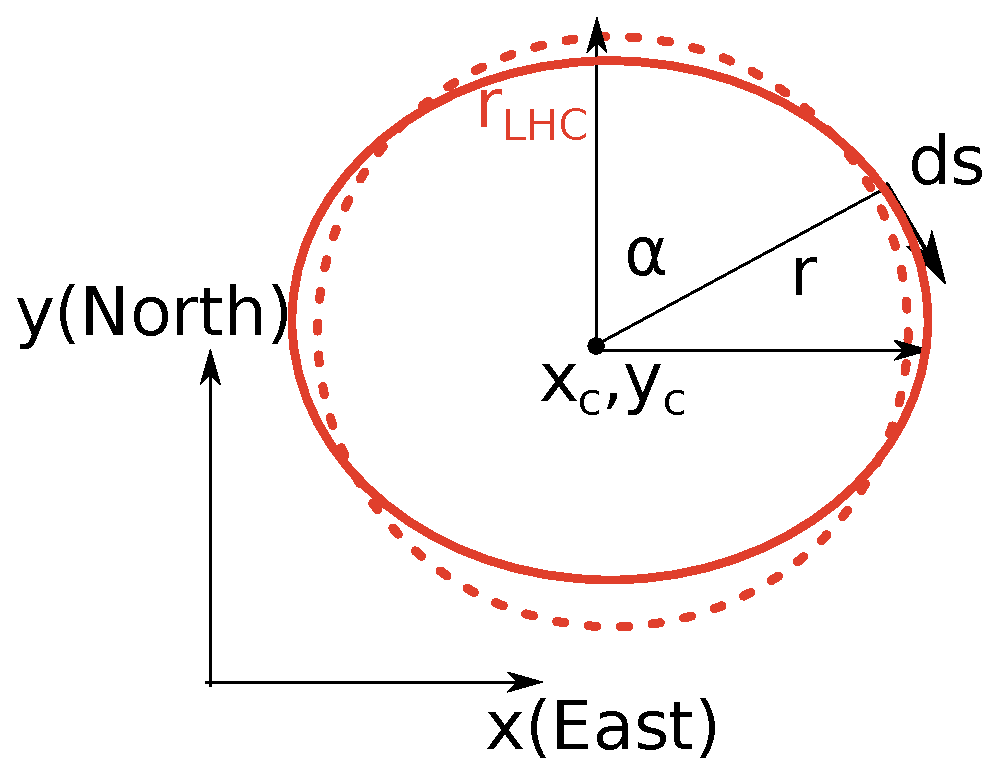
\includegraphics[width=\textwidth]{Ringschematically}
\end{figure}
The circumference of the LHC ring,  $\Delta L$, may be computed by a path
integral over the ring which is deformed from a perfect circle by the
deformation vector $\textbf{h}(x,y)$:
\begin{equation}
  L =\oint_{deformed ring} ds(x,y)
  \label{eq:int}
\end{equation}

We parameterize the path in terms of the angle $\alpha$. The infinitesimal path length $ds(x,y)$ , can then be
linked to $d\alpha$ by:
\begin{equation}
  \begin{split}
  ds(x,y)=|\textbf{x}_{c}(\alpha+d\alpha)+\textbf{h}(\alpha+d\alpha)-\textbf{x}_{c}(\alpha)+\textbf{h}(\alpha)|\\
  =&|d\textbf{x}_{c}(\alpha)+d\textbf{h}(\alpha)|\end{split}
\end{equation}

In terms of vector products $ds$ can be written as:
\begin{equation}\begin{split}
  d s =&
  \sqrt{[d\textbf{x}_{c}+d\textbf{h}]\cdot[d\textbf{x}_{c}+d\textbf{h}]}\\
  =& \sqrt{d\textbf{x}_{c} \cdot d\textbf{x}_{c}  +2
  d\textbf{x}_{c}\cdot d\textbf{h}+ d\textbf{h} \cdot d\textbf{h}} \end{split}
  \label{eq:2} \end{equation}

We now approximate the horizontal deformation $\textbf{h}$ as a
first order taylor series around the coordinate origin,
$\textbf{x}_{0}$:
\begin{equation}
  \textbf{h}(\textbf{x}_{c})\approx\textbf{h}\bigg|_{\textbf{x}_{0}} +
  \textbf{J}(\textbf{h})\bigg|_{\textbf{x}_{0}} [\textbf{x}_{c}-\textbf{x}_{0}]
\end{equation}
Where the Jacobian $\textbf{J}$ is composed of:
\begin{equation}
 \textbf{J}(\textbf{h})=\left[\begin{array}{cc}\frac{\partial
       h_{x}}{\partial x} & \frac{\partial h_{x}}{\partial y}\\\frac{\partial
       h_{y}}{\partial x} & \frac{\partial h_{y}}{\partial
       y}\end{array}\right]=\left[\begin{array}{cc}J_{11}
     &J_{12}\\J_{21}& J_{22}\end{array}\right]
\end{equation}

Building the difference vector between the locations associated with
$\alpha+d\alpha$ and $\alpha$ thus yield:
\begin{equation}
  d\textbf{h}(\alpha)=\textbf{J}(\textbf{h})\bigg|_{\textbf{x}_{0}} d\textbf{x}_{c}(\alpha)
\end{equation}

Substituting this in Eq. \ref{eq:2} yields:
\begin{equation}
ds = \sqrt{d\textbf{x}_{c}\cdot d\textbf{x}_{c} +2d\textbf{x}_{c}\cdot
  (\textbf{J}(\textbf{h})\bigg|_{\textbf{x}_{0}} d\textbf{x}_{c})
  +(\textbf{J}(\textbf{h})\bigg|_{\textbf{x}_{0}} d\textbf{x}_{c} )\cdot (\textbf{J}(\textbf{h})\bigg|_{\textbf{x}_{0}}) d\textbf{x}_{c})}
  \end{equation}

Since the expected horizontal deformations (order of mm) vary only
slightly over several 10's of km, the last term may be safely
discarded as it is scaled by the squares of these small horizontal gradients
In terms of $\alpha$, $d\textbf{x}_{c}$ is oriented tangential to the circle
and can be written as:
\begin{equation}
d\textbf{x}_{c}=r_{LHC}\left[\begin{array}{c}\cos\alpha\\-\sin\alpha\end{array}\right]d\alpha
\end{equation}

Subtituting the above in the integral of Eq. \ref{eq:int} and
evaluating the vector products yields:
\begin{equation}
  L =r_{LHC}\oint_{0}^{2\pi}
  \sqrt{1+J_{11}\cos^{2}\alpha+J_{22}\sin^{2}\alpha -(J_{12}+J_{21})\sin\alpha\cos\alpha} d\alpha 
\end{equation}

The above integral has similarities to the complete Elliptic integral
of the second kind, although an additional mixed term involving $\sin
\alpha\cos\alpha$ is present, and the bounds run to $2\pi$. In any
case no analytical solution exists for this integral, so one may
consider computing this numerically. However another approach would
be to linearize the state of the deformed ring against the undeformed
state (i.e. a perfect circle). This is generally justified as the
deformations are considered small relative to the ring geometry. Note
that in the the undeformed state, $\textbf{J}(\textbf{h})=\textbf{0}$,
so we can linearize around the situation where all $J_{ij}=0$.
The circumference can then be approximated as:
\begin{equation}
  L\approx L\bigg|_{circle}+\sum_{i=1}^{2}\sum_{j=1}^{2}\frac{\partial L
  }{\partial J_{ij}}\bigg|_{circle} J_{ij}=2\pi r_{LHC}+ \Delta L
  \end{equation}

Using Leibniz integral rule we can bring the differentation against
$J_{ij}$ within the integral. So one can write for the change of
circumference, $\Delta L$:
\begin{equation}
\Delta L = r_{LHC}\left[J_{11}\int_{0}^{2\pi} \cos^{2} d\alpha +
J_{22}\int_{0}^{2\pi} \sin^{2} d\alpha -
(J_{12}+J_{21})r_{LHC}\int_{0}^{2\pi} \cos\alpha\sin\alpha d\alpha\right]
\end{equation}
These trigonometric integrals can be evaluated analytically where the
last terms yields zero over the domain $0\ldots 2\pi$ such that:
\begin{equation}
  \Delta L = \frac{\pi r_{LHC}}{2 } (J_{11} + J_{22})=\frac{\pi
    r_{LHC}}{2 } \left(\frac{\partial h_{x}}{\partial
    x}+\frac{\partial h_{y}}{\partial y}\right)\bigg|_{\textbf{x}_{0}}
  \label{eq:dL}
\end{equation}


Circumference changes caused by horizontal Earth deformations are
thus linearly proportional to the radius of the ring. from a signal to
noise perspective this means that large rings have clearly an
advantage when loading signals are to be recovered. To compute
circumference changes according to Eq. \ref{eq:dL}, we will (only)
need the compute the  2 gradients $\frac{\partial h_{x}}{\partial x},\frac{\partial h_{y}}{\partial y}$ at the ring's
center. For surface loading phenomena this will be the topic of the
next sections.

\subsection{Hydrology and atmospheric induced LHC circumference
  changes from GRACE data}

GRACE results are commony provided in terms of spherical harmonic
Stokes coefficients which describe the Earth's potential field. Most
variability of the gravity field is caused by mass redistribution
close to the Earth's surface (i.e. a  thin shell). Using a thin shell
assumption together with an elastic Earth model, geoid changes,
horizonta/vertical deformations can be computed from those Stokes
coefficients.\\

A surface load (in equivalent water height),$T(\theta,\lambda)$, at
longitude $\lambda$ and colatitude $\theta$,can be be described in
terms of a spherical harmonic expansion:
\begin{equation}
  T(\theta,\lambda)=a\sum_{n=0}^{\infty}\sum_{m=-n}^{n} T_{nm} \bar{Y}(\theta,\lambda)
\end{equation}

Where $a$ is the mean Earth radius, and the spherical harmonic functions are normalized
$4\pi$ -'geodesy-style'. Which means that:

\begin{equation}
\bar{Y}_{nm}=\left\{\begin{array}{c} N_{nm}P_{nm}(\cos \theta)\cos m\lambda,\; m\ge0\\N_{n|m|}P_{n|m|}(\cos \theta)\sin |m|\lambda,\; m<0\end{array}\right.
\end{equation}
Where $P_{nm}$ are the associated Legendre functions, without a
Condon-Shortly Phase applied. The normalization factor is defined as:
\begin{equation}
N_{nm}=\sqrt{(2-\delta_{0m})(2n+1)\frac{(n-m)!}{(n+m)!}}
\end{equation}

In practice, the combined product $N_{n|m|}P_{n|m|}$ may be  directly computed by
recursion, as $P_{nm}$ will be numerically unstable for higher degrees
$n$.

In that form the following orrhogonality property holds:
\begin{equation}
\oint \bar{Y}_{nm}(\omega)\bar{Y}_{n'm'}(\omega)d\omega=4\pi \delta_{nn'}\delta_{mm'}
  \end{equation}


Horizontal deformation can be comuted from the surface loading
coefficients $T_{nm}$ by (see e.g. Eq. 4.3 Dissertation Rietbroek 2014):

\begin{equation}
\textbf{h}(\theta,\lambda)=\frac{3a\rho_{w}}{\rho_{e}}\sum_{n=1}^{\infty}\sum_{m=-n}^{n}\frac{l'_{n}}{2n+1}\left[\begin{array}{c}
    \frac{\partial \bar{Y}_{nm}}{\sin \theta \partial
      d\lambda}\\-\frac{\partial \bar{Y}_{nm}}{\partial \theta}\end{array}\right]T_{nm}
\end{equation}
The Spherically symmetric Non-rotating Elastic Isotropic (SNREI) Earth model is contained within the so-called load Love
numbers, $l'_{n}$,which are only dependent on the degree, and describe
the horizontal deformation response due to a surface load.
For the circumference changes we need the derivative of those
contributions. Noting that:
\begin{eqnarray}
\partial x &=& a\sin\theta \partial \lambda\\
\partial y &=& -a\partial \theta\\
\end{eqnarray}
and simplifying the notation by introducing the surface gradient
operator:
\begin{equation}
  \nabla_{\Omega}=\left[\begin{array}{c}\frac{\partial}{\sin\theta
        \partial \lambda}\\\frac{\partial}{\partial \theta} \end{array}\right]
  \end{equation}

yields a cicrumference change of:

\begin{equation}
  \Delta L =\frac{\pi r_{LHC}}{2} \frac{3\rho_{w}}{\rho_{e}}\sum_{n=1}^{\infty}\sum_{m=-n}^{n}\frac{l'_{n}}{2n+1}\left[\nabla_{\Omega} \cdot
  (\nabla_{\Omega} \bar{Y}_{nm})\right]T_{nm}
\end{equation}

The terms with the surface gradient operator can furthermore be
simplified to ease its numerical computation. Realizing that the
surface spherical harmonics obey the following differenttial equation:

\begin{equation}
  r^{2}\nabla^{2} \bar{Y}_{nm}= -n(n+1)\bar{Y}_{nm}
\end{equation}
which in spherical coordinates is:
\begin{equation}
  \frac{\cos\theta}{\sin\theta}\frac{\partial \bar{Y}_{nm}}{\partial
    \theta}+\frac{\partial^{2}\bar{Y}_{nm}}{\partial\theta^{2}}+\frac{\partial^{2} \bar{Y}_{nm}}{\sin^{2}\theta\partial \lambda^{2}}= -n(n+1)\bar{Y}_{nm}
\end{equation}

So:
\begin{equation}
  \Delta L =\frac{\pi r_{LHC}}{2}
  \frac{3\rho_{w}}{\rho_{e}}\sum_{n=1}^{\infty}\sum_{m=-n}^{n}\frac{-l'_{n}}{2n+1}\left[
    \frac{\cos\theta}{\sin\theta}\frac{\partial \bar{Y}_{nm}}{\partial
      \theta} +n(n+1)\bar{Y}_{nm}\right]T_{nm}
  \label{eq:jacT}
\end{equation}



The spherical harmonic and its derivative can be computed numerically
for the center position of the ring.

Using thin shell assumptions, the fully normalized Stokes coefficients (relative to a
static field) provided by
GRACE, $\delta C_{nm}$, can be linked to the Surface laoding
coefficients by:
\begin{equation}
\delta C_{nm} = \frac{1+k'_{n}}{2n+1}\frac{3\rho_{w}}{\rho_{e}}
T_{nm},\; n>0
\end{equation}

The load Love number $k'_{n}$ now describes the change in potential of
the Earth upon a forcing by a surface load.
So equation \ref{eq:jacT} can also be written in terms of Stokes
coefficient (anomalies)
\begin{equation}
  \Delta L =\frac{\pi r_{LHC}}{2}
  \sum_{n=1}^{\infty}\sum_{m=-n}^{n}\frac{-l'_{n}}{1+k'_{n}}\left[
    \frac{\cos\theta}{\sin\theta}\frac{\partial \bar{Y}_{nm}}{\partial
    \theta} +n(n+1)\bar{Y}_{nm}\right]\delta C_{nm}
\label{eq:jacpot}
\end{equation}




TODONOTE: Consistent treatment of reference systems (i.e. degree 1 contributions)











\subsection{LHC circumference changes due to water level changes in Lake Geneva}

\appendix
\section{Deformation relative to a deforming surface point}
The deformation in an 'isomorphic' reference frame induced by a surface load on an elastic earth can be described in the local East, North, Up axis system as:
\begin{equation}
\textbf{d}(\theta,\lambda)=\frac{3a\rho_{w}}{\rho_{e}}\sum_{n=1}^{\infty}\sum_{m=-n}^{n}\frac{1}{2n+1}\left[\begin{array}{c}
    l'_{n}\frac{\partial \bar{Y}_{nm}}{\sin \theta \partial
      d\lambda}\\-l'_{n}\frac{\partial \bar{Y}_{nm}}{\partial \theta}\\h'_{n}\bar{Y}_{nm}\end{array}\right]T_{nm}
\end{equation}

The choice of the degree 1 load Love numbers (i.e. $h'_{1},l'_{1}$) determines which isomorphic reference is used to describe the deformation.

Now if we want to shift the reference frame origin, to follow that of a surface point $\lambda_{0},\theta_{0}$, we need to express this offset first in terms of cartesian coordinates apply the shift and then rotate it back in the local ENU system. On a spherical Earth the rotation matrix is described as follows:
\begin{equation}
\textbf{R}_{xyz\rightarrow ENU}(\theta,\lambda)=\left[\begin{array}{ccc}-\sin\lambda&\cos\lambda&0\\-\cos\lambda\cos\theta&-\sin\lambda\cos\theta&\sin\theta\\\cos\lambda\sin\theta&\sin\lambda\sin\theta&\cos\theta\end{array}\right]
\end{equation}

Furthermore, one should note that the above rotation matrix can also be written in terms of degree 1 spherical harmonics and its derivatives:

\begin{equation}
\textbf{R}_{xyz\rightarrow ENU}(\theta,\lambda)=\frac{1}{\sqrt{3}}\left[\begin{array}{ccc}\frac{\partial \bar{Y}_{11}}{\sin \theta \partial
      d\lambda}&\frac{\partial \bar{Y}_{1-1}}{\sin \theta \partial d\lambda}&0\\
      -\frac{\partial \bar{Y}_{11}}{\partial \theta}&-\frac{\partial \bar{Y}_{1-1}}{\partial \theta}&-\frac{\partial \bar{Y}_{10}}{\partial \theta}\\
      \bar{Y}_{11}&\bar{Y}_{1-1}&\bar{Y}_{10}\\
      \end{array}\right]
\end{equation}

We can shift the deformation $\textbf{d}$ to a frame which moves with the deformation at the reference surface point, $\textbf{d}_{0}=\textbf{d}(\lambda_{0},\theta_{0})$
\begin{equation}
\tilde{\textbf{d}}=\textbf{d}-\textbf{R}(\theta,\lambda)\textbf{R}^{T}(\theta_{0},\lambda_{0})\textbf{d}_{0}
\end{equation}

It can be shown that this expression for this relative deformation is independent of the chosen (isomorphic) reference frame (and thus the associated reference frame origin of the degree 1 Love numbers are irrelavant). To see this note that the degree 1 contributions to the relative  deformation above can be written in terms of the rotation matrix int he cartesian frame:
\begin{equation}
\tilde{\textbf{d}}(\theta,\lambda,n=1)=\frac{\sqrt{3}a\rho_{w}}{\rho_{e}}\left[\boldsymbol{\Lambda}\textbf{R}(\theta,\lambda)-\textbf{R}(\theta,\lambda)\textbf{R}^{T}(\theta_{0},\lambda_{0})\boldsymbol{\Lambda}\textbf{R}(\theta_{0},\lambda_{0})\right]\left[\begin{array}{c}T_{11}\\T_{1-1}\\T_{10}\\\end{array}\right]
\end{equation}

where the load Love numbers are contained within the diagonal matrix:
\begin{equation}
\boldsymbol{\Lambda}=\left[\begin{array}{ccc}l_{1}'&0&0\\0&l_{1}'&0\\0&0&h_{1}'\\\end{array}\right]
\end{equation}

A shifted reference frame would be accomplished by adding a unit diagonal matrix scaled by an isomorphic frame parameter $\alpha$:
\begin{equation}
\boldsymbol{\Lambda}^{*}=\boldsymbol{\Lambda}+\alpha\boldsymbol{I}
\end{equation}

The frame independence can be tested by substituting $\boldsymbol{\Lambda}^{*}$ which will result in the same expression as using $\boldsymbol{\Lambda}$, when the orthogonality of the rotation matrices is exploited.


% make Bibliography
%% \bibliography{roelofsrefsauto}
%% \bibliographystyle{abbrvnat}
%\bibliographystyle{plainnat}
%\bibliographystyle{authordate1}
\end{document}

